\documentclass[multi=tikzpicture,border=7pt]{standalone}
\usepackage{ctex}
\usepackage{amsmath}
\usepackage{bm}
\usepackage{tikz}
\usetikzlibrary{arrows.meta,calc,decorations.pathmorphing,patterns,positioning,angles,quotes}
\tikzset{
  axis/.style={->,>=Stealth,thick}, force/.style={->,>=Stealth,very thick},
  flow/.style={->,>=Stealth,thick,blue!70!black}, dim/.style={<->,>=Stealth,thin},
  current/.style={->,>=Stealth,very thick,purple!75!black},
  body/.style={draw=black,fill=blue!10,thick}
}
\begin{document}

% 01 question-01
\begin{tikzpicture}[x=1cm,y=1cm]
  \begin{scope}
    \draw[very thick] (-1.8,0)--(-1.55,3.4) (1.8,0)--(1.55,3.4) (-1.8,0)--(1.8,0);
    \fill[blue!15] (-1.65,.35) rectangle (1.65,2.7);
    \draw[blue!70!black,thick] (-1.65,2.7)--(1.65,2.7);
    \filldraw[fill=blue!55,thick] (-.45,1.8) rectangle (.45,2.35);
    \draw[flow] (0,1.75)--++(0,-.85) node[right]{$a$};
    \draw[very thick] (-2.3,-.25)--(2.3,-.25)--(1.85,-1.35)--(-1.85,-1.35)--cycle;
    \draw (0,-.78) circle(.38); \draw[->] (0,-.78)--(.22,-.55);
    \node at (0,-1.75){密度为 $\rho_3$ 的物体下沉};
  \end{scope}
  \begin{scope}[shift={(6,0)}]
    \draw[very thick] (-1.8,0)--(-1.55,3.4) (1.8,0)--(1.55,3.4) (-1.8,0)--(1.8,0);
    \fill[blue!15] (-1.65,.35) rectangle (1.65,2.7);
    \draw[blue!70!black,thick] (-1.65,2.7)--(1.65,2.7);
    \draw[red!65!black,very thick,decorate,decoration={coil,aspect=.25,segment length=3pt,amplitude=2pt}]
       (0,2.68)--(0,.35);
    \draw[very thick] (-2.3,-.25)--(2.3,-.25)--(1.85,-1.35)--(-1.85,-1.35)--cycle;
    \draw (0,-.78) circle(.38); \draw[->] (0,-.78)--(.22,-.55);
    \draw[dim] (2.15,.35)--(2.15,2.7) node[midway,right]{$h$};
    \node at (0,-1.75){链条下端在容器底部堆积};
  \end{scope}
\end{tikzpicture}

% 02 solution-01
\begin{tikzpicture}[x=1cm,y=1cm]
  \begin{scope}
    \filldraw[fill=blue!35,thick] (0,1.2) rectangle (1,2);
    \draw[force] (.5,1.2)--++(0,-1.15) node[right]{$m_3g$};
    \draw[force,orange!80!black] (.5,2)--++(0,.85) node[right]{$F_b=\rho_1Vg$};
    \draw[flow] (1.45,1.8)--++(0,-.8) node[right]{$a$};
    \node at (.5,-.35){物体受力};
  \end{scope}
  \begin{scope}[shift={(4.8,0)}]
    \draw[very thick] (-1.8,0)--(-1.55,3.1) (1.8,0)--(1.55,3.1) (-1.8,0)--(1.8,0);
    \fill[blue!12] (-1.65,.3) rectangle (1.65,2.55);
    \filldraw[fill=blue!45,thick] (-.35,1.25) rectangle (.35,1.85);
    \draw[flow] (.7,1.75)--++(0,-.75) node[right]{物体下移 $\mathrm dz$};
    \draw[flow,red!70!black] (-.7,1.0)--++(0,.75) node[left]{等体积水上移};
    \node[align=center] at (0,-.55){质心位移对应的有效质量\\$m_3-\rho_1V$};
  \end{scope}
  \begin{scope}[shift={(9,0)}]
\draw[axis] (0,0)--(4.4,0) node[right]{$t/t_f$};\draw[axis] (0,0)--(0,3.7) node[above]{$N$};
\draw[dashed] (0,1.5)--(4.1,1.5) node[right]{$M_4g$};
\draw[blue!70!black,thick,domain=0:1,samples=75] plot({3*\x},{.5+3*\x*\x});
\draw[blue!70!black,thick] (3,1.5)--(4,1.5);\draw[dashed] (3,3.5)--(3,1.5);
\draw[fill=white] (3,3.5) circle(2pt);\fill (3,1.5) circle(2pt);
\node[above] at (3,3.5){$M_4g+2m_4g\eta_4^2$};\node[below] at (3,0){$1$};\node[left] at (0,.5){$M_4g-m_4g\eta_4^2$};
\node at (2,-1){末段落底前趋于峰值，落完后回到总重};
\end{scope}
\end{tikzpicture}

% 03 question-02
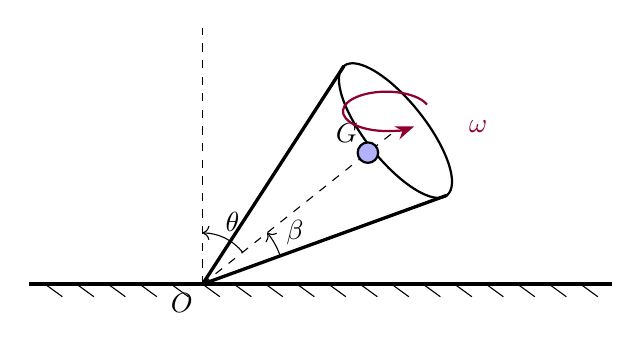
\begin{tikzpicture}[x=1cm,y=1cm]
  \draw[very thick] (-2.2,0)--(5.2,0);
  \foreach \x in {-2,-1.6,...,5}{\draw (\x,0)--++(.22,-.16);}
  \coordinate (O) at (0,0); \coordinate (C) at (2.45,1.95);
  \coordinate (V) at (0,3.25);
  \coordinate (B1) at ($(C)+(128.5:1.05)$);
  \coordinate (B2) at ($(C)+(-51.5:1.05)$);
  \draw[dashed] (O)--(C);
  \draw[very thick] (O)--(B1) (O)--(B2);
  \begin{scope}[shift={(C)},rotate=128.5]
    \draw[thick] (0,0) ellipse[x radius=1.05,y radius=.38];
  \end{scope}
  \draw[dashed] (O)--(V);
  \filldraw[fill=blue!30,thick] (2.1,1.67) circle(.13) node[above left]{$G$};
  \draw pic[draw,->,"$\theta$",angle radius=.65cm,angle eccentricity=1.35]{angle=C--O--V};
  \draw pic[draw,->,"$\beta$",angle radius=1.05cm,angle eccentricity=1.28]{angle=B2--O--C};
  \node[below left] at (O){$O$};
  \draw[flow,purple!75!black] (2.85,2.28) arc[start angle=20,end angle=310,x radius=.55,y radius=.25];
  \node[purple!75!black] at (3.5,2.0){$\omega$};
\end{tikzpicture}

% 04 solution-02
\begin{tikzpicture}[x=1cm,y=1cm]
\begin{scope}
\draw[thick] (-1,0)--(4,0);\coordinate (G) at (1.1,1.8);\fill (G) circle(2pt) node[right]{$G$};\fill (0,0) circle(2pt) node[below]{$O$};\draw[thick] (0,0)--(1.47,2.4);
\draw[force] (G)--++(0,-1.3) node[right]{$Mg$};\draw[force,orange!80!black] (0,0)--(0,1.4) node[left]{$N$};\draw[force,red!70!black] (0,0)--(1,0) node[below]{$f$};
\draw[dashed] (0,0)--(0,2.7);\node at (.25,.65){$\theta$};\node at (1.4,-.8){(a) 倾倒时质心加速度决定 $f,N$};
\end{scope}
\begin{scope}[shift={(7,0)}]
\draw[axis] (0,0)--(0,3.1) node[above]{$\boldsymbol\Omega$};\draw[force,blue!70!black] (0,0)--(1.8,2.5) node[right]{$\boldsymbol L_s=I_s\omega\hat{\boldsymbol e}_3$};
\node[red!70!black] at (0,0){$\otimes$};\node[red!70!black,left] at (-.2,-.3){$\boldsymbol\tau$ 入纸面};
\draw[->,blue!70!black] (.7,2.8) arc(30:280:.65 and .25);
\node[align=center] at (1,-1){(b) 轴矢量在纸面内，力矩垂直纸面\\$\boldsymbol\tau=\boldsymbol\Omega\times\boldsymbol L_s$};
\end{scope}\end{tikzpicture}

% 05 question-03
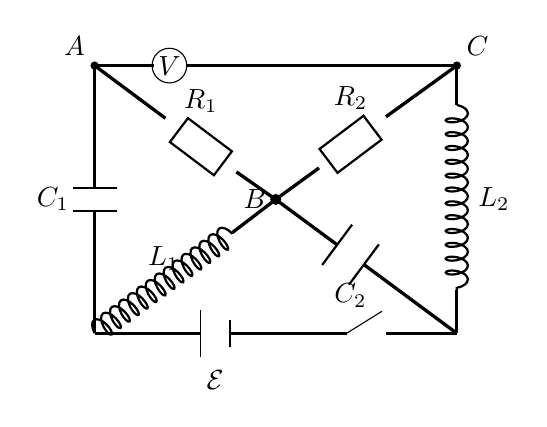
\begin{tikzpicture}[x=1cm,y=1cm]
  \coordinate (A) at (0,3.4); \coordinate (C) at (4.6,3.4);
  \coordinate (D) at (0,0); \coordinate (E) at (4.6,0); \coordinate (B) at (2.3,1.7);
  \draw[very thick] (A)--(.75,3.4); \draw (.95,3.4) circle(.22) node{$V$}; \draw[very thick] (1.17,3.4)--(C);
  \draw[very thick] (A)--(0,1.85) (0,1.55)--(D);\draw[thick] (-.28,1.85)--(.28,1.85) (-.28,1.55)--(.28,1.55); \node[left] at (-.2,1.7){$C_1$};
  \draw[very thick] (C)--(4.6,2.9); \draw[thick,decorate,decoration={coil,aspect=.45,segment length=5pt,amplitude=4pt}] (4.6,2.9)--(4.6,.55); \draw[very thick] (4.6,.55)--(E); \node[right] at (4.75,1.7){$L_2$};
  \draw[very thick] (D)--(1.35,0); \draw (1.35,-.3)--(1.35,.3) (1.72,-.17)--(1.72,.17); \node[below] at (1.53,-.35){$\mathcal E$}; \draw[very thick] (1.72,0)--(3.2,0); \draw (3.2,0)--(3.65,.28); \draw[very thick] (3.7,0)--(E);
  \draw[thick,decorate,decoration={coil,aspect=.42,segment length=4pt,amplitude=4pt}] (D)--(1.75,1.28); \draw[very thick] (1.75,1.28)--(B); \node[left] at (1.2,.95){$L_1$};
  \draw[very thick] (A)--(.9,2.73); \draw[fill=white,thick,rotate around={-37:(1.35,2.37)}] (1.0,2.18) rectangle (1.7,2.56); \draw[very thick] (1.8,2.05)--(B); \node[above] at (1.35,2.68){$R_1$};
  \draw[very thick] (B)--(2.85,2.1); \draw[fill=white,thick,rotate around={37:(3.25,2.4)}] (2.9,2.21) rectangle (3.6,2.59); \draw[very thick] (3.7,2.75)--(C); \node[above] at (3.25,2.72){$R_2$};
  \draw[very thick] (B)--(3.08,1.124) (3.42,.873)--(E);\draw[thick] (2.89,.868)--(3.27,1.38) (3.23,.617)--(3.61,1.129); \node[below] at (3.25,.75){$C_2$};\fill (B) circle(2pt);
  \fill (A) circle(1.5pt) node[above left]{$A$}; \fill (B) circle(1.5pt) node[left]{$B$}; \fill (C) circle(1.5pt) node[above right]{$C$};
\end{tikzpicture}

% 06 solution-03
\begin{tikzpicture}[x=1cm,y=1cm]
\tikzset{res/.style={decorate,decoration={zigzag,segment length=4pt,amplitude=2pt}},coil/.style={decorate,decoration={coil,aspect=.4,segment length=5pt,amplitude=4pt}}}
\coordinate (A) at (0,2.4);\coordinate (B) at (3,2.4);\coordinate (C) at (6,2.4);\coordinate (D) at (0,0);\coordinate (E) at (6,0);
\draw[thick,res] (A)--(B) node[midway,above]{$R_1$};\draw[thick,res] (B)--(C) node[midway,above]{$R_2$};
\draw[thick] (A)--(0,1.35) (0,1.05)--(D);\draw[thick] (-.3,1.35)--(.3,1.35) (-.3,1.05)--(.3,1.05);\node[left] at (-.3,1.2){$C_1$};
\draw[thick,coil] (D)--(B) node[midway,below right]{$L_1$};\draw[thick,coil] (C)--(E) node[midway,right]{$L_2$};
\draw[thick] (B)--(4.32,1.344) (4.68,1.056)--(E);\draw[thick] (4.12,1.094)--(4.52,1.594) (4.48,.806)--(4.88,1.306);\node[right] at (4.8,1.2){$C_2$};
\foreach \P/\lab in {A/A,B/B,C/C}{\fill (\P) circle(2pt) node[above=.3cm]{$\lab$};}
\draw[flow,red!70!black] (2.6,3.2)--(.4,3.2) node[midway,above]{$i_1(0^+)$};\draw[flow,red!70!black] (3.4,3.2)--(5.6,3.2) node[midway,above]{$i_2(0^+)$};
\node[align=center] at (3,-.8){左回路 $B\to A\to D\to B$；右回路 $B\to C\to E\to B$\\只共用节点 $B$，没有共用支路；电源支路已断开};\end{tikzpicture}

% 07 question-04
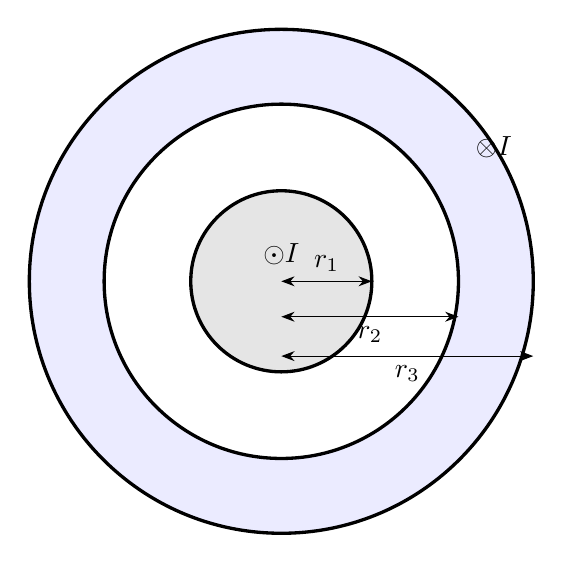
\begin{tikzpicture}[x=1cm,y=1cm]
  \fill[blue!8] (0,0) circle(3.2); \fill[white] (0,0) circle(2.25); \fill[gray!20] (0,0) circle(1.15);
  \draw[very thick] (0,0) circle(1.15) circle(2.25) circle(3.2);
  \draw[dim] (0,0)--(1.15,0) node[midway,above]{$r_1$};
  \draw[dim] (0,-.45)--(2.25,-.45) node[midway,below]{$r_2$};
  \draw[dim] (0,-.95)--(3.2,-.95) node[midway,below]{$r_3$};
  \node at (0,.35){$\odot I$};
  \node at (2.7,1.7){$\otimes I$};
\end{tikzpicture}

% 08 solution-04
\begin{tikzpicture}[x=1cm,y=1cm]
  \draw[axis] (-.2,0)--(7,0) node[right]{$r$};
  \draw[axis] (0,-.2)--(0,4.2) node[above]{$B(r)$};
  \draw[blue!70!black,very thick] (0,0)--(1.5,2.6);
  \draw[blue!70!black,very thick,domain=1.5:3.5,samples=80] plot(\x,{3.9/\x});
  \draw[blue!70!black,very thick,domain=3.5:5.6,samples=80] plot(\x,{3.9/\x*(5.6*5.6-\x*\x)/(5.6*5.6-3.5*3.5)});
  \draw[blue!70!black,very thick] (5.6,0)--(6.7,0);
  \foreach \x/\lab in {1.5/r_1,3.5/r_2,5.6/r_3}{\draw[dashed] (\x,0)--(\x,3.2);\node[below] at (\x,0){$\lab$};}
  \node[blue!70!black] at (2.8,3.2){均匀体电流};
  \begin{scope}[shift={(9,0)}]
    \draw[axis] (-.2,0)--(6.7,0) node[right]{$r$};
    \draw[axis] (0,-.2)--(0,4.2) node[above]{$B(r)$};
    \draw[red!75!black,very thick] (0,0)--(1.5,0);
    \draw[red!75!black,very thick,domain=1.5:3.5,samples=80] plot(\x,{3.9/\x});
    \draw[red!75!black,very thick] (3.5,0)--(6.5,0);
    \foreach \x/\lab in {1.5/r_1,3.5/r_2}{\draw[dashed] (\x,0)--(\x,3.2);\node[below] at (\x,0){$\lab$};}
    \node[red!75!black] at (2.9,3.2){理想表面电流};
  \end{scope}
\end{tikzpicture}

% 09 question-05
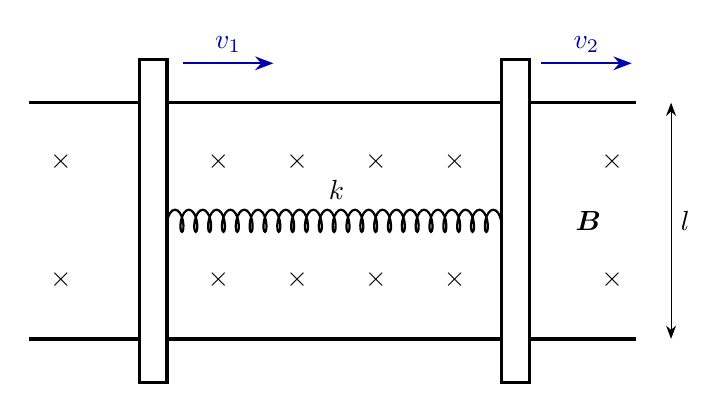
\begin{tikzpicture}[x=1cm,y=1cm]
  \draw[very thick] (-.4,3)--(7.3,3) (-.4,0)--(7.3,0);
  \draw[very thick,fill=white] (1.0,-.55) rectangle (1.35,3.55);
  \draw[very thick,fill=white] (5.6,-.55) rectangle (5.95,3.55);
  \draw[thick,decorate,decoration={coil,aspect=.4,segment length=5pt,amplitude=4pt}] (1.35,1.5)--(5.6,1.5);
  \node[above] at (3.5,1.65){$k$};
  \foreach \x in {0,2,3,4,5,7}{\node at (\x,2.25){$\times$};\node at (\x,.75){$\times$};}
  \node at (6.7,1.5){$\bm B$};
  \draw[flow] (1.55,3.5)--++(1.15,0) node[midway,above]{$v_1$};
  \draw[flow] (6.1,3.5)--++(1.15,0) node[midway,above]{$v_2$};
  \draw[dim] (7.75,0)--(7.75,3) node[midway,right]{$l$};
\end{tikzpicture}

% 10 solution-05
\begin{tikzpicture}[x=.9cm,y=2cm]
\begin{scope}
\draw[axis] (0,0)--(8,0) node[right]{$u$};\draw[axis] (0,-.1)--(0,1.3) node[above]{$v_1/(J/m)$};
\draw[blue!70!black,thick] (0,.5)--(7.7,.5) node[right]{严格约束};
\draw[red!70!black,thick,domain=0:7.7,samples=150] plot(\x,{.5*(1+cos(2*\x*180/pi))});
\node[red!70!black] at (4,-.4){仅电感：示例 $B^2l^2/(mL)=k/m$};\end{scope}
\begin{scope}[shift={(10,0)}]
\draw[axis] (0,0)--(8,0) node[right]{$u$};\draw[axis] (0,-.1)--(0,1.3) node[above]{$v_1/(J/m)$};
\draw[purple!70!black,thick,domain=0:7.7,samples=180] plot(\x,{.5*(1+(3+sqrt(17))/(2*sqrt(17))*cos(sqrt((5+sqrt(17))/2)*\x*180/pi)-(3-sqrt(17))/(2*sqrt(17))*cos(sqrt((5-sqrt(17))/2)*\x*180/pi))});
\node at (4,-.4){含电容：准确双频与初值};\end{scope}\end{tikzpicture}

% 11 question-06
\begin{tikzpicture}[x=1cm,y=1cm]
  \draw[very thick] (0,0) rectangle (10,3.6);
  \draw[very thick] (2.5,0)--(2.5,3.6) (5,0)--(5,3.6) (7.5,0)--(7.5,3.6);
  \draw[red!70!black,line width=3pt] (2.5,.25)--(2.5,3.35);
  \draw[green!50!black,line width=3pt] (5,.25)--(5,3.35);
  \draw[blue!70!black,line width=3pt] (7.5,.25)--(7.5,3.35);
  \node at (1.25,1.8){$A$\\$1\,\mathrm{mol\ He}$};
  \node at (3.75,1.8){$B$\\$\mathrm{He}$};
  \node at (6.25,1.8){$C$\\$\mathrm{He+N_2}$};
  \node at (8.75,1.8){$D$\\$1\,\mathrm{mol\ N_2}$};
  \draw[fill=orange!20,thick] (-1.25,.7) rectangle (0,2.9); \node[align=center] at (-.63,1.8){热源\\$T_0$};
  \node[red!70!black,below] at (2.5,0){自由绝热};
  \node[green!50!black,below,align=center] at (5,0){固定绝热\\半透膜};
  \node[blue!70!black,below] at (7.5,0){自由绝热};
\end{tikzpicture}

% 12 solution-06
\begin{tikzpicture}[x=1cm,y=1cm]
  \draw[very thick] (0,0) rectangle (14,3.5);
  \draw[very thick] (3.3,0)--(3.3,3.5) (6.6,0)--(6.6,3.5) (9.8,0)--(9.8,3.5);
  \node[font=\small] at (1.65,2.45){$V_A=(1-y)V_0$};
  \node[font=\small] at (4.95,2.45){$V_B=(1+y)V_0$};
  \node[font=\small] at (8.2,2.45){$V_C=(1-x)V_0$};
  \node[font=\small] at (11.9,2.45){$V_D=(1+x)V_0$};
  \node at (1.65,1.1){$T_A=T_0$};
  \node at (4.95,1.1){$T_B=T_1$};
  \node at (8.2,1.1){$T_C=T_1$};
  \node at (11.9,1.1){$T_D=T_2$};
  \draw[flow,red!75!black] (11.2,-.85)--(11.9,-.05) node[midway,right]{$Q$};
  \draw[flow,purple!75!black] (5.8,3.95)--(6.6,3.55) node[midway,above]{氦气可通过};
\end{tikzpicture}

% 13 question-07
\begin{tikzpicture}[x=1cm,y=1cm]
  \draw[very thick] (0,0) circle(3.5) circle(2.35);
  \foreach \a in {0,30,...,330}{
    \draw[thick] ({2.92*cos(\a)},{2.92*sin(\a)}) ellipse[x radius=.22,y radius=.58,rotate=\a];
  }
  \draw[dim] (0,0)--(2.92,0) node[midway,above]{$r$};
  \draw[dim] (2.92,-.7)--(3.5,-.7) node[midway,below]{$a$};
  \node at (0,0){$N$ 个等间距绝热活塞};
\end{tikzpicture}

% 14 solution-07
\begin{tikzpicture}[x=1cm,y=1cm]
  \draw[very thick] (-.5,0)--(10.5,0) (-.5,2.5)--(10.5,2.5);
  \foreach \x/\lab in {1/n-1,4/n,7/n+1}{
    \draw[very thick,fill=blue!12] (\x,-.25) rectangle ({\x+.18},2.75);
    \node[below] at ({\x+.09},-.3){$\lab$};
  }
  \draw[dim] (1.18,3.15)--(4,3.15) node[midway,above]{$d+x_n-x_{n-1}$};
  \draw[dim] (4.18,3.15)--(7,3.15) node[midway,above]{$d+x_{n+1}-x_n$};
  \draw[force,red!75!black] (4.1,1.25)--++(1.0,0) node[above]{$p_{n-1,n}A$};
  \draw[force,orange!80!black] (4.1,1.25)--++(-1.0,0) node[above]{$p_{n,n+1}A$};
  \draw[flow,purple!75!black] (1.1,-1.05)--(7.1,-1.05) node[midway,below]{相位逐格增加 $\phi$};
\end{tikzpicture}

% 15 question-08
\begin{tikzpicture}[x=.05cm,y=.05cm]
\draw[axis] (-125,0)--(25,0) node[right]{$p_x$};\draw[axis] (0,-50)--(0,70) node[above]{$p_y$};
\draw[force,blue!70!black] (0,0)--(-24.7,-24.9) node[below]{$\mu^+$};\draw[force,green!50!black] (0,0)--(-104.1,5.3) node[left]{$\nu$};\draw[force,orange!80!black] (0,0)--(-14.2,50.1) node[above]{$\mathrm{Jet\ 1}$};
\node[align=center] at (-50,-75){图示测得的横向动量，单位 $\mathrm{GeV}/c$\\纵向 $p_z^{(\nu)}$ 待质量壳约束确定};\end{tikzpicture}

% 16 solution-08
\begin{tikzpicture}[x=1cm,y=1cm]
\draw[axis] (-5.3,0)--(3.4,0) node[right]{$z/(50\,\mathrm{GeV}/c)$};\draw[axis] (0,0)--(0,4.8) node[above]{$m^2/(3000\,\mathrm{GeV}^2)$};
\draw[blue!70!black,thick,domain=-5:3,samples=160] plot(\x,{sqrt(1383.86)/30*sqrt(4.34596+\x*\x)-1.6262+0.413333333*\x});
\draw[red!70!black,thick] (-5,2.15472)--(3,2.15472) node[right]{$m_W^2$};
\fill (-3.765874,2.15472) circle(2pt) node[above left]{$z=-188.2937$};\fill (1.479064,2.15472) circle(2pt) node[above right]{$z=73.9532$};
\node[align=center] at (-1,-1){蓝线直接计算 $2(E_\mu E_\nu-\boldsymbol p_\mu\cdot\boldsymbol p_\nu)$\\各交点代回未平方方程均成立};\end{tikzpicture}

\end{document}
